\documentclass[tikz,border=10pt]{standalone}
\usepackage{tikz}
\usepackage{tikz-feynman}
\usetikzlibrary{graphs}
\begin{document}
    
    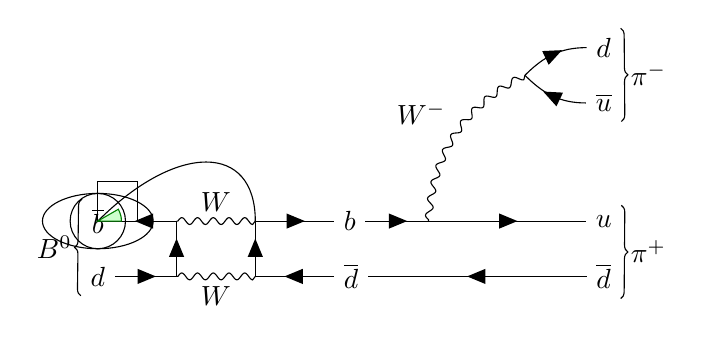
\begin{tikzpicture}
        \begin{feynman}
        \vertex (a1) {\(\overline b\)};
        \vertex[right=1cm of a1] (a2);
        \vertex[right=1cm of a2] (a3);
        \vertex[right=1cm of a3] (a4) {\(b\)};
        \vertex[right=1cm of a4] (a5);
        \vertex[right=2cm of a5] (a6) {\(u\)};
        \vertex[below=2em of a1] (b1) {\(d\)};
        \vertex[right=1cm of b1] (b2);
        \vertex[right=1cm of b2] (b3);
        \vertex[right=1cm of b3] (b4) {\(\overline d\)};
        \vertex[below=2em of a6] (b5) {\(\overline d\)};
        \vertex[above=of a6] (c1) {\(\overline u\)};
        \vertex[above=2em of c1] (c3) {\(d\)};
        \vertex at ($(c1)!0.5!(c3) - (1cm, 0)$) (c2);
        \diagram* {
        {[edges=fermion]
        (b1) -- (b2) -- (a2) -- (a1),
        (b5) -- (b4) -- (b3) -- (a3) -- (a4) -- (a5) -- (a6),
        },
        (a2) -- [boson, edge label=\(W\)] (a3),
        (b2) -- [boson, edge label'=\(W\)] (b3),
        (c1) -- [fermion, out=180, in=-45] (c2) -- [fermion, out=45, in=180] (c3),
        (a5) -- [boson, bend left, edge label=\(W^{-}\)] (c2),
        };
        \draw [decoration={brace}, decorate] (b1.south west) -- (a1.north west)
        node [pos=0.5, left] {\(B^{0}\)};
        \draw [decoration={brace}, decorate] (c3.north east) -- (c1.south east)
        node [pos=0.5, right] {\(\pi^{-}\)};
        \draw [decoration={brace}, decorate] (a6.north east) -- (b5.south east)
        node [pos=0.5, right] {\(\pi^{+}\)};
        \end{feynman}

        \draw (0,0) circle (10pt);     %画一个圆心在原点,半径为10pt的圆;
        \draw (0,0) .. controls (1,1) and (2,1) .. (2,0);       %画一个起点为(0,0),终点为(2,0),控制点为(1,1),(2,1)的贝塞尔曲线;
        \draw (0,0) ellipse (20pt and 10pt);       %画一个中心在原点,长轴、短轴分别为20pt和10pt的椭圆;
        \draw (0,0) rectangle (0.5,0.5);       %画一个从(0,0)到(0.5,0.5)的矩形
        \filldraw[fill=green!20!white, draw=green!50!black](0,0) -- (3mm,0mm) arc (0:30:3mm) -- cycle;
        %画一个扇形,并填充,扇形的边色和填充色的透明度不同。
        \end{tikzpicture}
\end{document}